\pdfobjcompresslevel 0
\documentclass[
11pt, % The default document font size, options: 10pt, 11pt, 12pt
%oneside, % Two side (alternating margins) for binding by default, uncomment to switch to one side
%chapterinoneline,% Have the chapter title next to the number in one single line
french, % ngerman for German
singlespacing, % Single line spacing, alternatives: onehalfspacing or doublespacing
%draft, % Uncomment to enable draft mode (no pictures, no links, overfull hboxes indicated)
%nolistspacing, % If the document is onehalfspacing or doublespacing, uncomment this to set spacing in lists to single
%liststotoc, % Uncomment to add the list of figures/tables/etc to the table of contents
%toctotoc, % Uncomment to add the main table of contents to the table of contents
%parskip, % Uncomment to add space between paragraphs
%nohyperref, % Uncomment to not load the hyperref package
headsepline, % Uncomment to get a line under the header
]{MastersDoctoralThesis} % The class file specifying the document structure

\usepackage[utf8]{inputenc}
\DeclareUnicodeCharacter{2010}{-}
%\usepackage[french]{babel}
\usepackage{amsmath}
\usepackage{lmodern}
\usepackage{amsfonts}
\usepackage{amssymb}
\usepackage{graphicx}
\usepackage{color}
\usepackage{xcolor}
\usepackage{url}
\usepackage{subcaption}
\usepackage{glossaries}
\usepackage{hyperref}
\usepackage{palatino} % Use the Palatino font by default
\usepackage{minitoc}


%\usepackage[backend=bibtex,style=authoryear,natbib=true]{biblatex} % Use the bibtex backend with the authoryear citation style (which resembles APA)
 
%\addbibresource{biblio.bib} % The filename of the bibliography
 
\usepackage[autostyle=true]{csquotes} % Required to generate language-dependent quotes in the bibliography

%-------------------------------
% COLOR SETTINGS


\definecolor{olivegreen}{RGB}{207,228,50}
\definecolor{briquered}{RGB}{155,61,34}
\definecolor{semilightblue}{RGB}{52,153,255}
\definecolor{pinkyred}{RGB}{255,103,103}

\definecolor{plum}{HTML}{92268F}
\definecolor{oliveGreen}{HTML}{007E00}

\definecolor{rose_cochon}{HTML}{CE6363}
\definecolor{bleu_random}{HTML}{002CA6}
\definecolor{violet_cool}{HTML}{4E005C}
\definecolor{vert_fonce}{HTML}{005413}

\definecolor{brique}{HTML}{B9655E}
\definecolor{vert_turquoise}{HTML}{53C36A}
\definecolor{bleu_window}{HTML}{3E9BDA}


\definecolor{bleu_transparent}{HTML}{0088B1}
%-------------------------------


 
\usepackage[textsize=footnotesize,obeyFinal]{todonotes}
\setlength{\marginparwidth}{2.5cm}
\newcommand{\note}[1]{\todo[color=orange!80]{#1}\ }
\newcommand{\inline}[1]{\todo[color=orange!80, inline]{#1}}

\newcommand{\resume}[1]{
	\begin{colbox}{D0D0D0}
	\textbf{Résumé}
	
	#1
	\end{colbox}
}
	
\newsavebox{\selvestebox}
\newenvironment{colbox}[1]
  {\newcommand\colboxcolor{#1}%
   \begin{lrbox}{\selvestebox}%
   \begin{minipage}{\dimexpr\columnwidth-2\fboxsep\relax}}
  {\end{minipage}\end{lrbox}%
   \begin{center}
   \colorbox[HTML]{\colboxcolor}{\usebox{\selvestebox}}
   \end{center}}


\DeclareMathOperator*{\argmin}{arg\,min}


\newcommand{\largeurGroupeDense}{0.28}
\newcommand{\groupcharac}[4]{
\begin{figure}[#4]
	\centering
	\begin{subfigure}{\largeurGroupeDense\linewidth}
		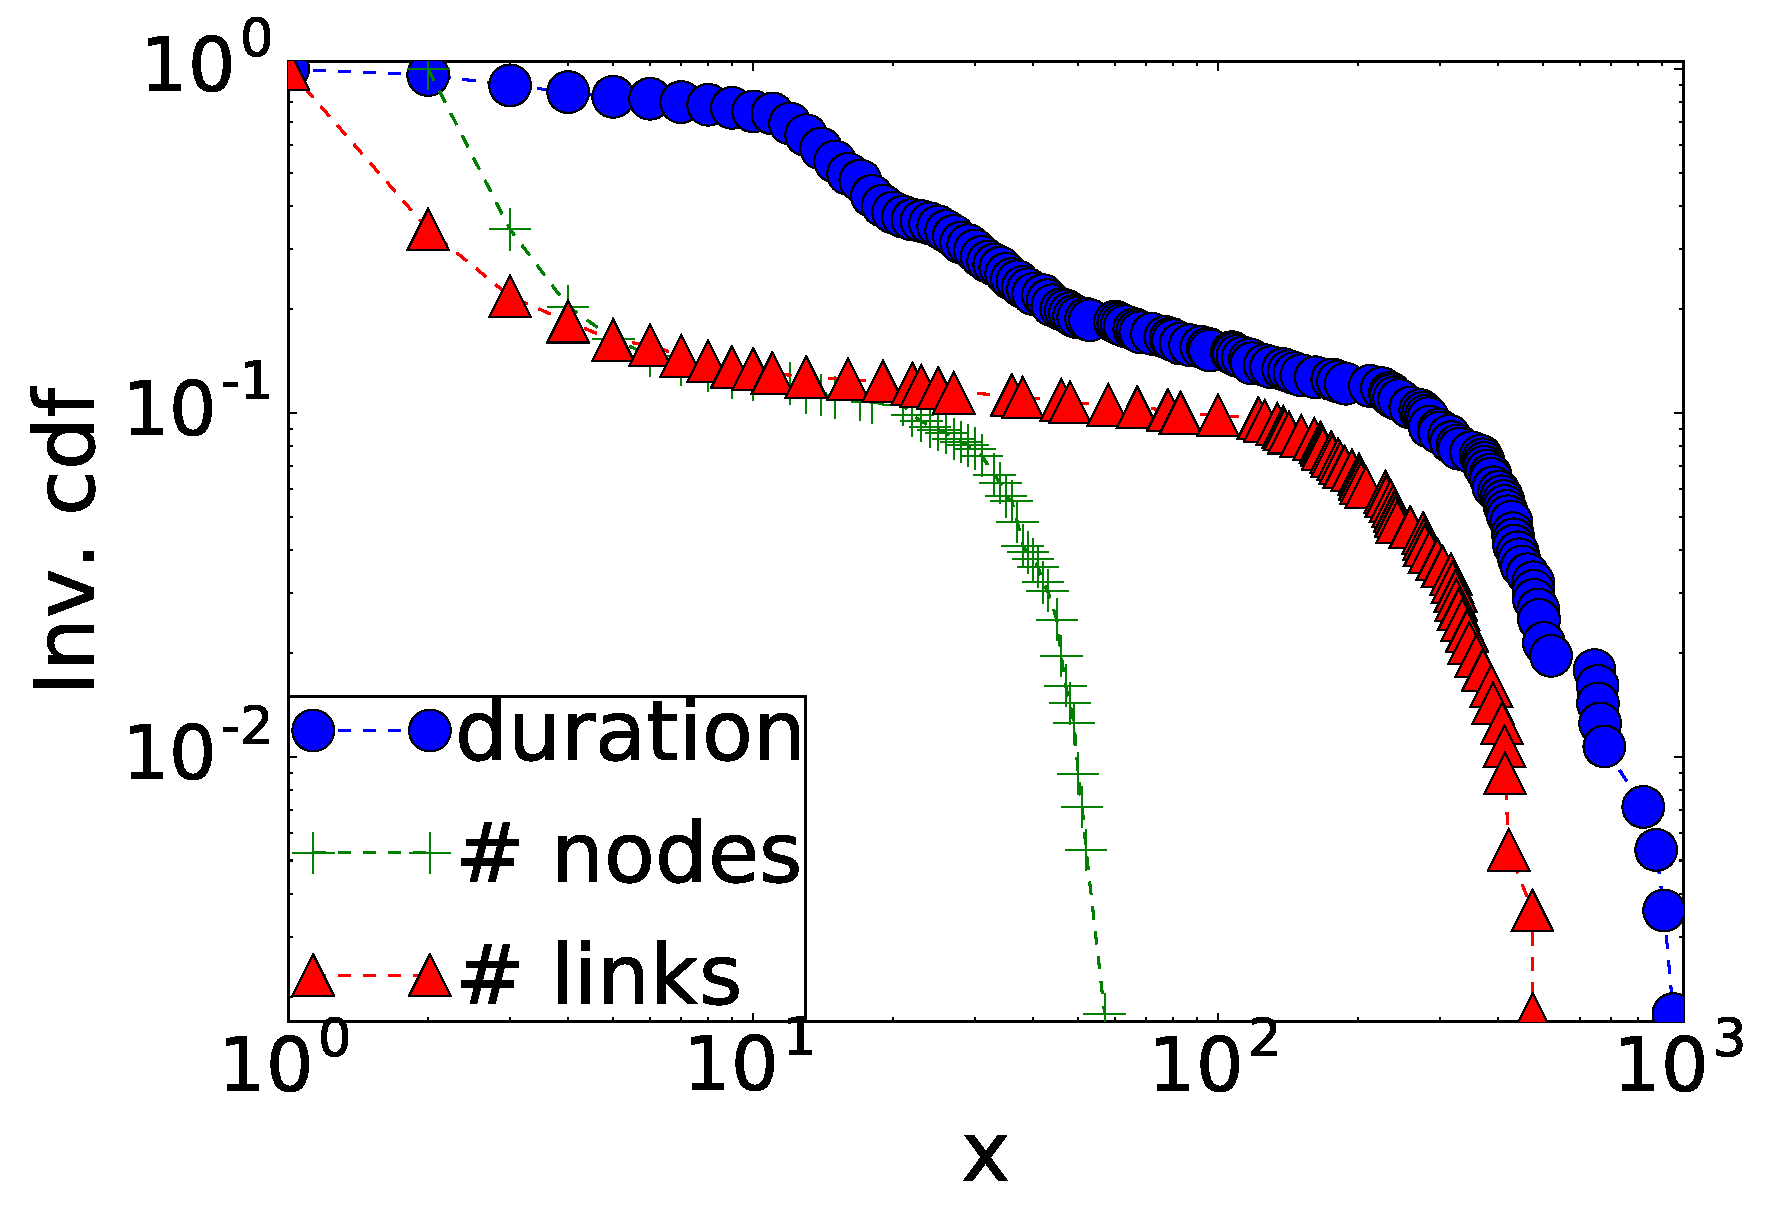
\includegraphics[width=\linewidth]{img/GroupeDense/#1/filter/Distrib_avant_filtre_best}
	\end{subfigure}\hspace{0.03\linewidth}
	\begin{subfigure}{\largeurGroupeDense\linewidth}
		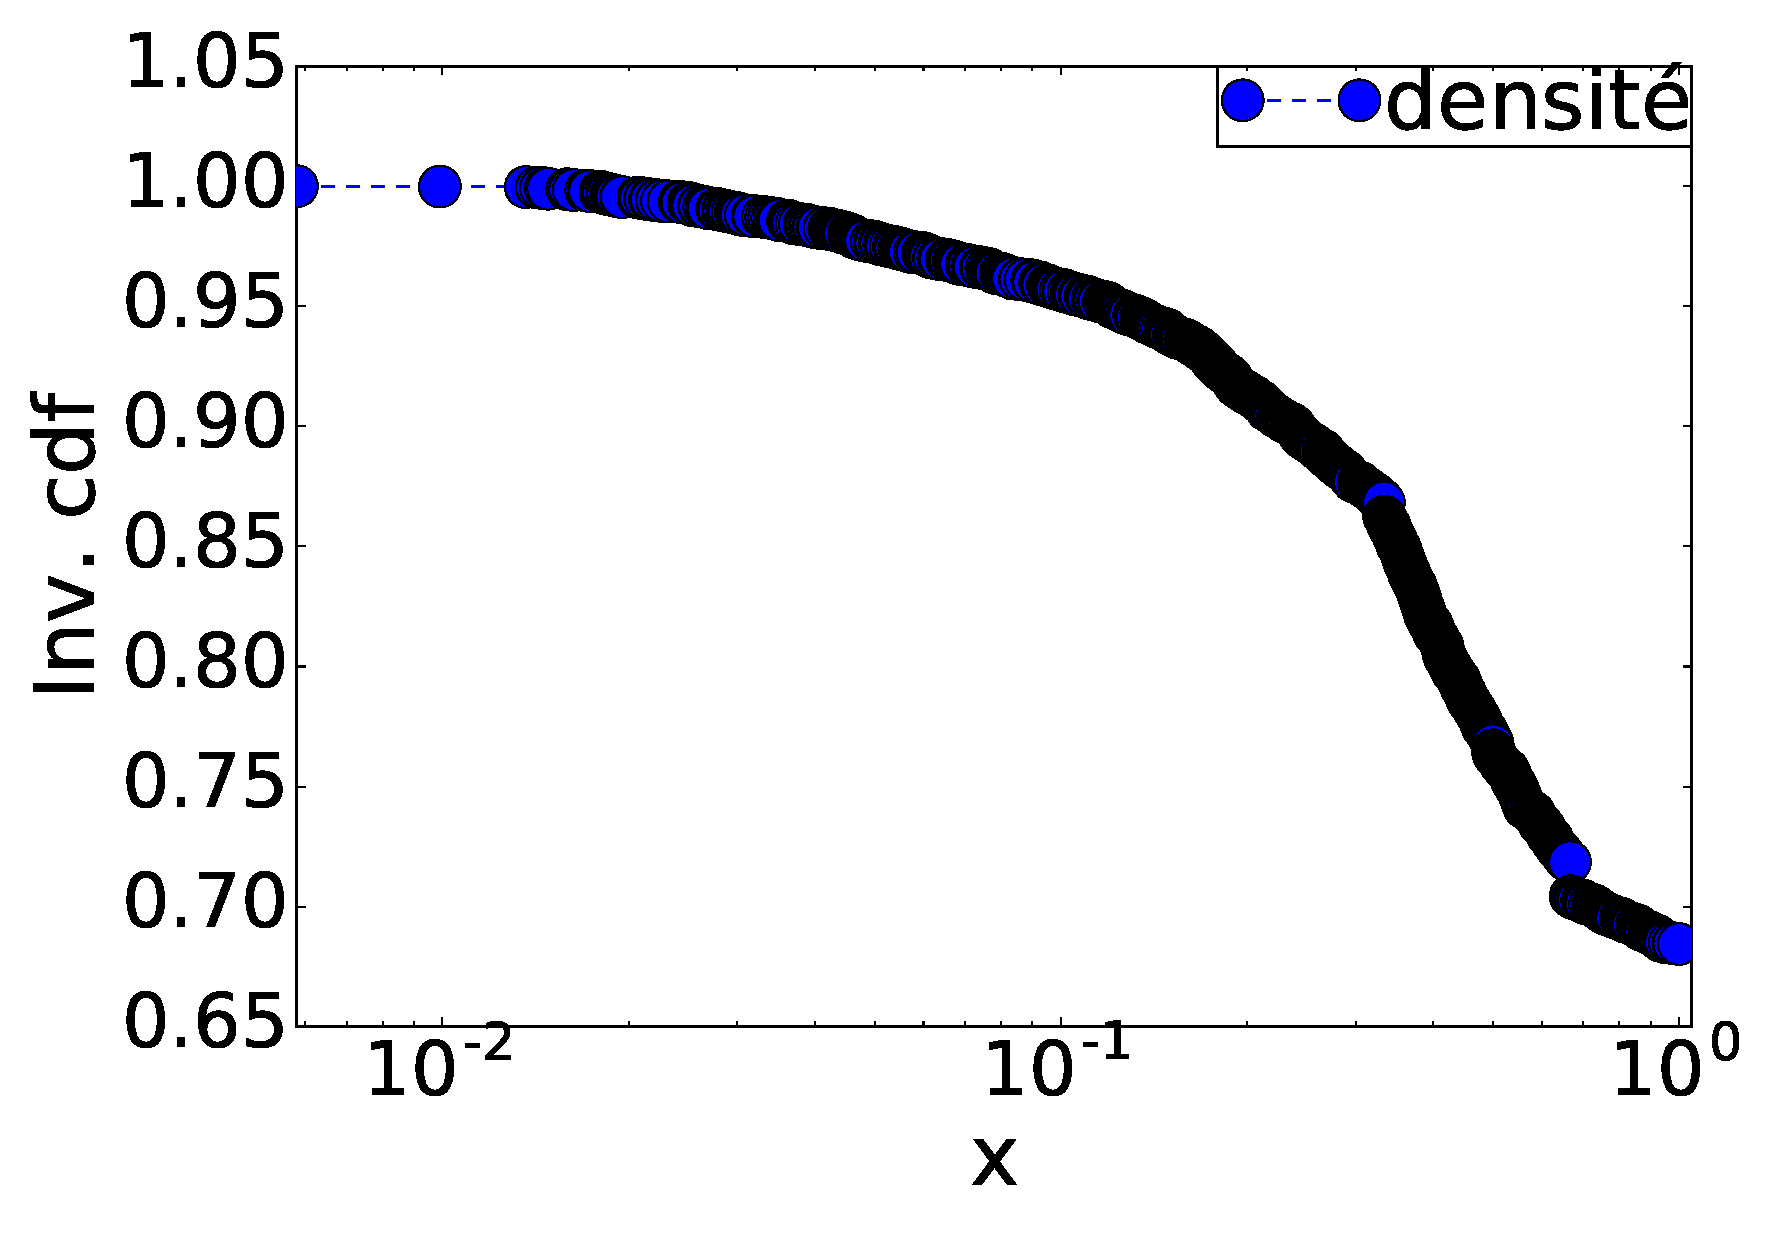
\includegraphics[width=\linewidth]{img/GroupeDense/#1/filter/Distrib_avant_dens.eps}
	\end{subfigure}
	\caption{Distribution cumulative inverse du nombre de liens, de n\oe uds et de la durée en (A) et de la densité en (B) pour les candidats trouvés par la méthode de Louvain dans le jeu de données #2.}
	\label{fig:distri_group_#3}
\end{figure}
}

\newcommand{\groupsPerNode}[4]{
	\begin{figure}[#4]
	\centering
	
	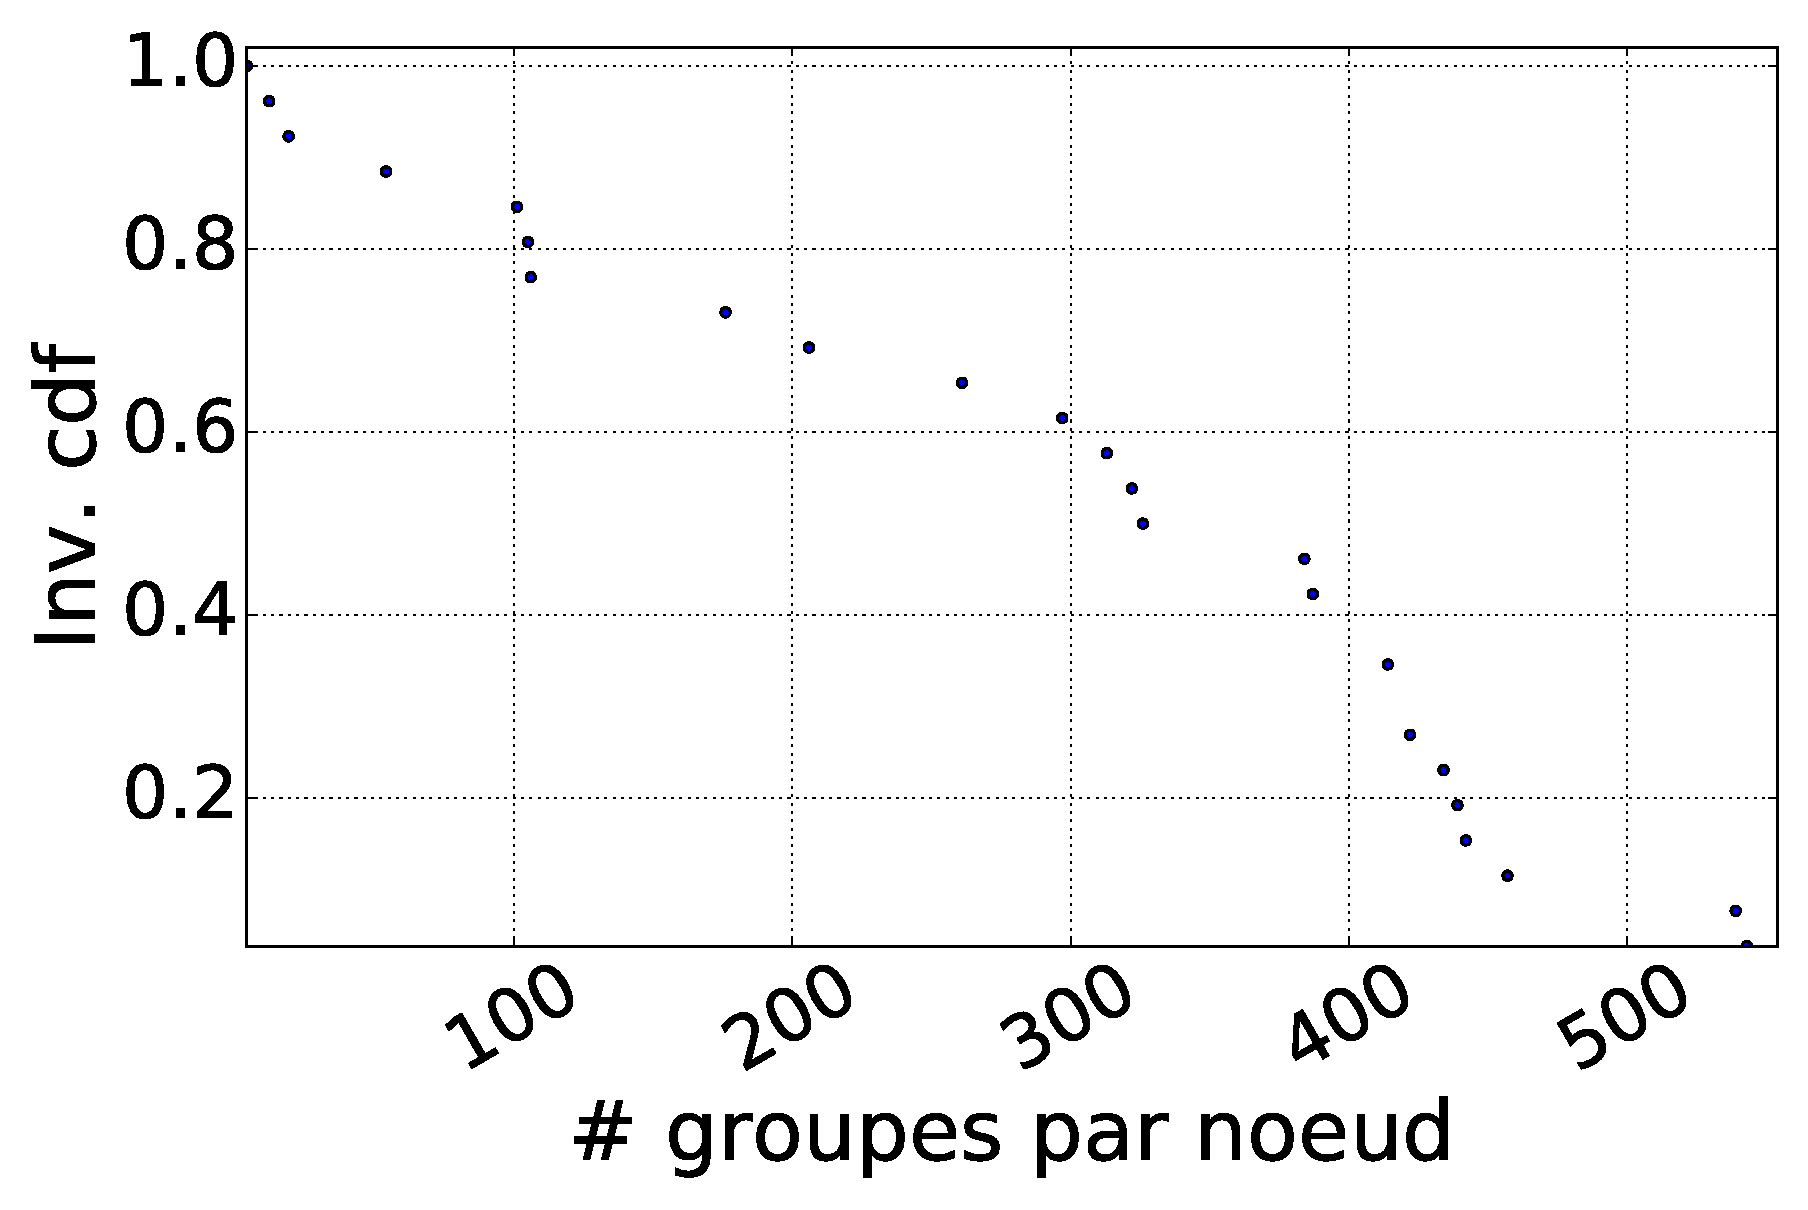
\includegraphics[width=0.5\linewidth]{img/GroupeDense/#1/filter/Prop_node.eps}
	\caption{Distribution cumulative inverse du nombre de groupes pertinent auquel un n\oe ud appartient dans le jeu de données #2.}
	\label{fig:ditribnodes_#3}
	\end{figure}
}

\newcommand{\percentile}[4]{
	\begin{figure}[#4]
	\centering
	
	\begin{subfigure}{\largeurGroupeDense\linewidth}
		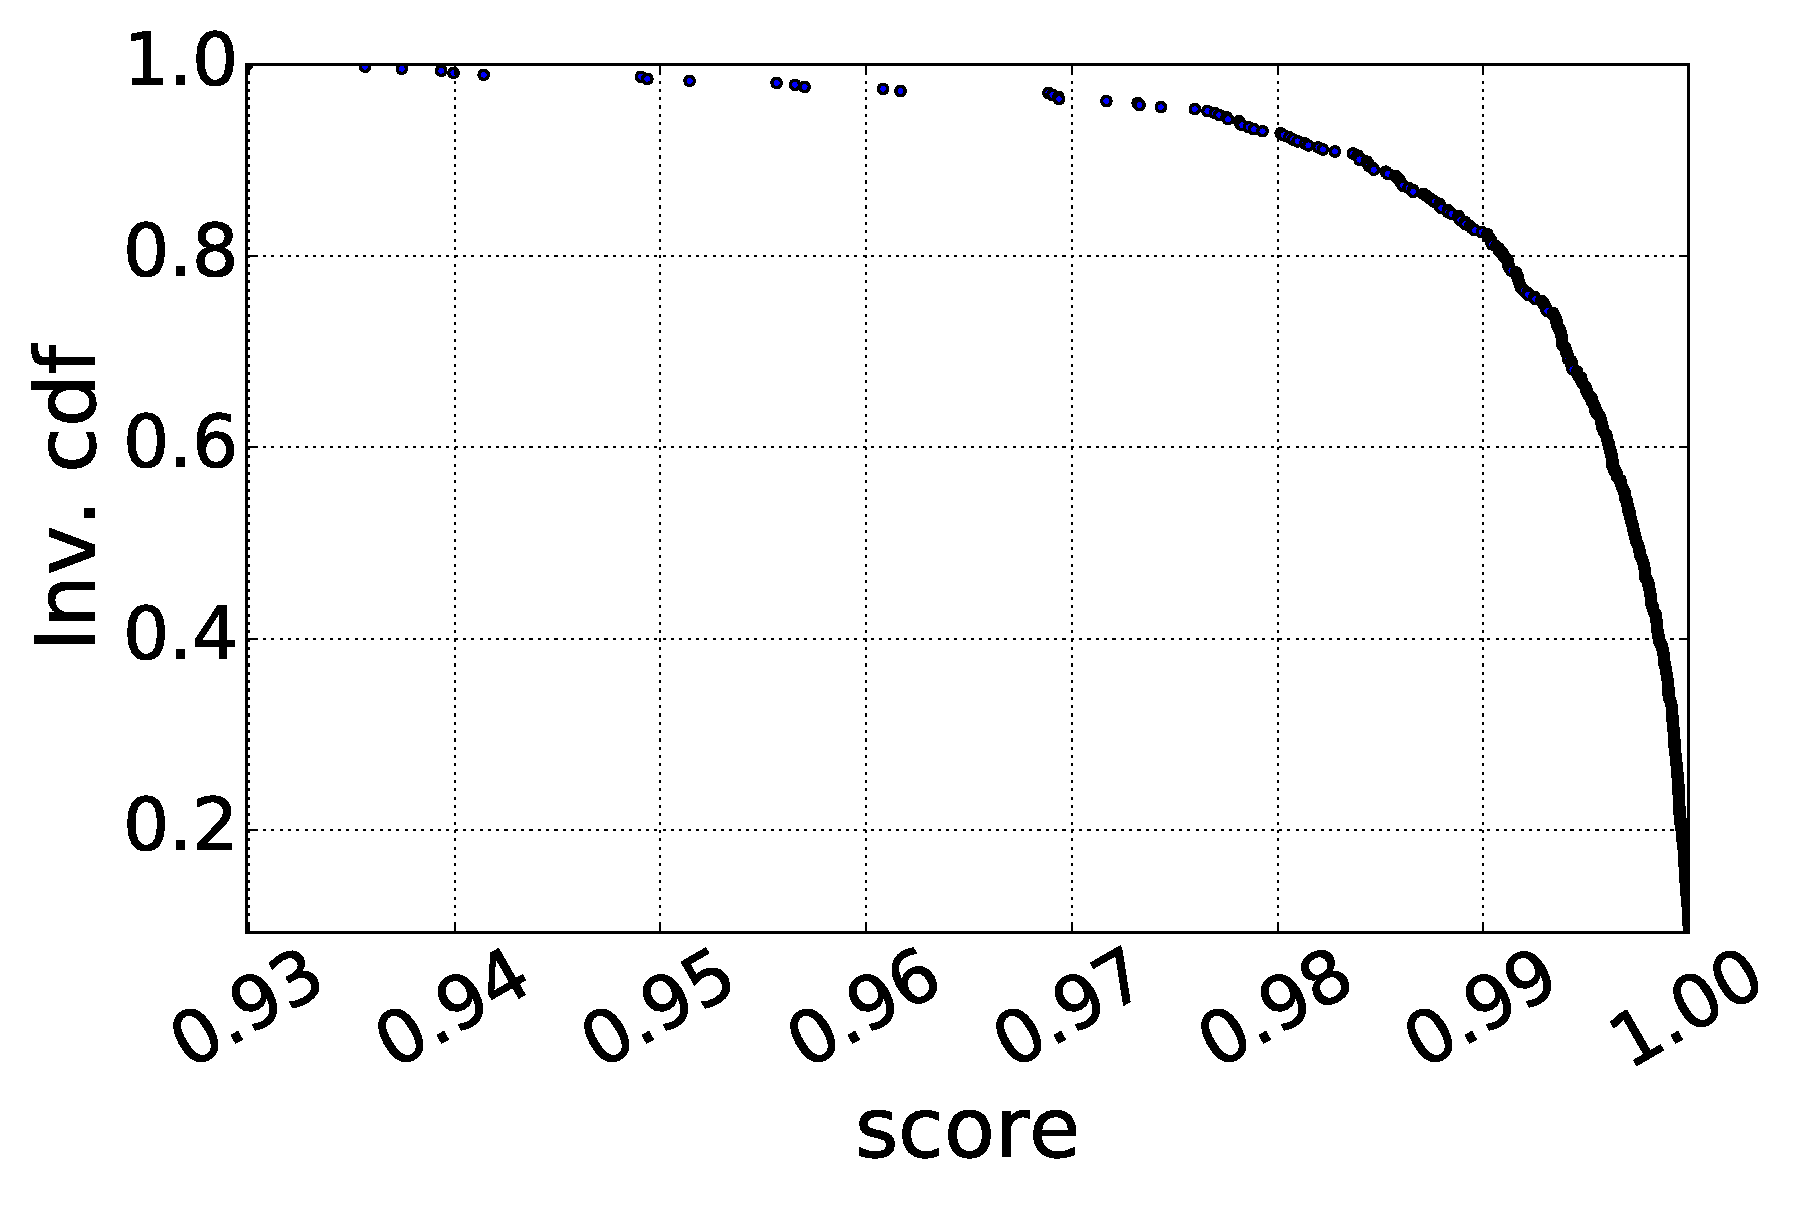
\includegraphics[width=\linewidth]{img/GroupeDense/#1/Percentil/Distribution_percentil_FixDuration_top155.eps}
		\caption{Temps de début: $p_{d\acute{e}but}$}
	\end{subfigure}\hfill
	\begin{subfigure}{\largeurGroupeDense\linewidth}
		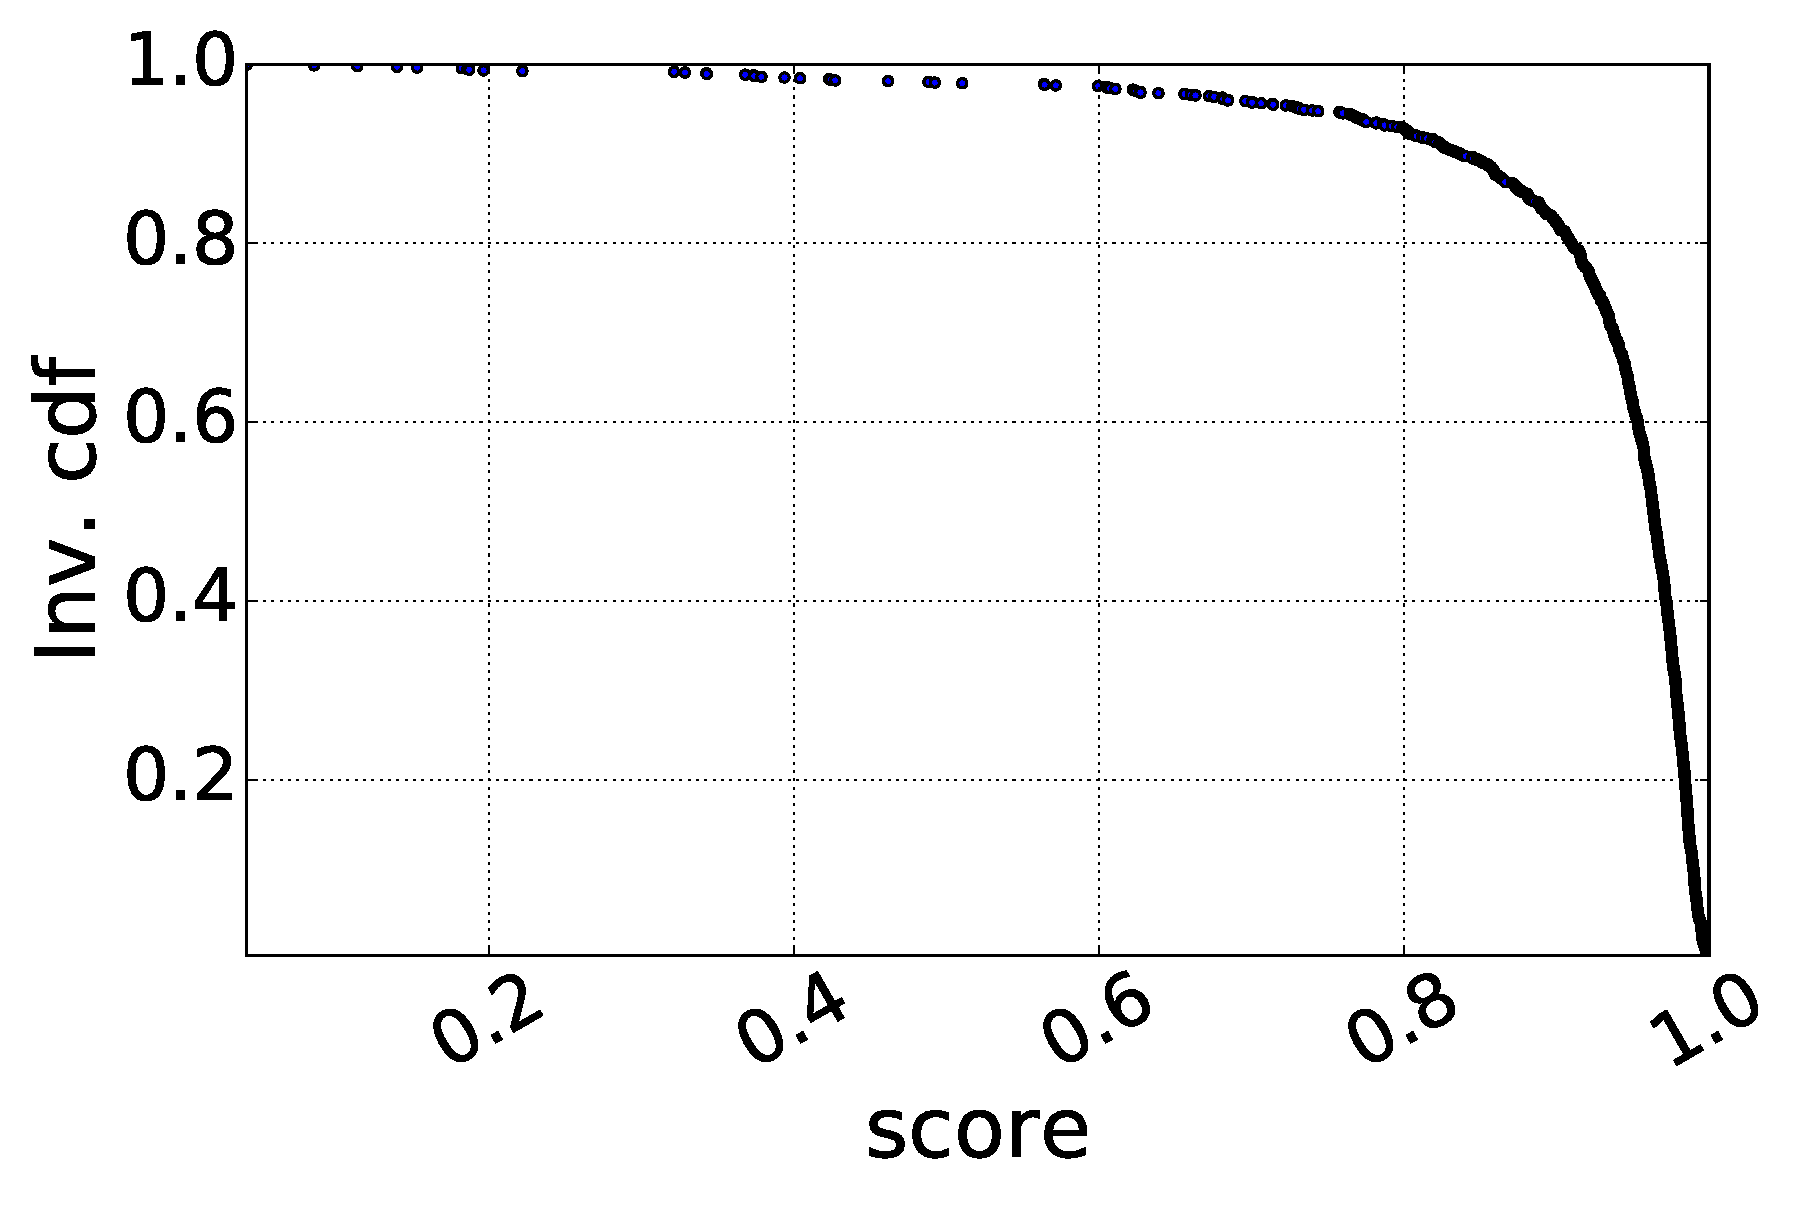
\includegraphics[width=\linewidth]{img/GroupeDense/#1/Percentil/Distribution_percentil_FixTime_top155.eps}
		\caption{Durée: $p_{dur\acute{e}e}$}
	\end{subfigure}\hfill
	\begin{subfigure}{\largeurGroupeDense\linewidth}
		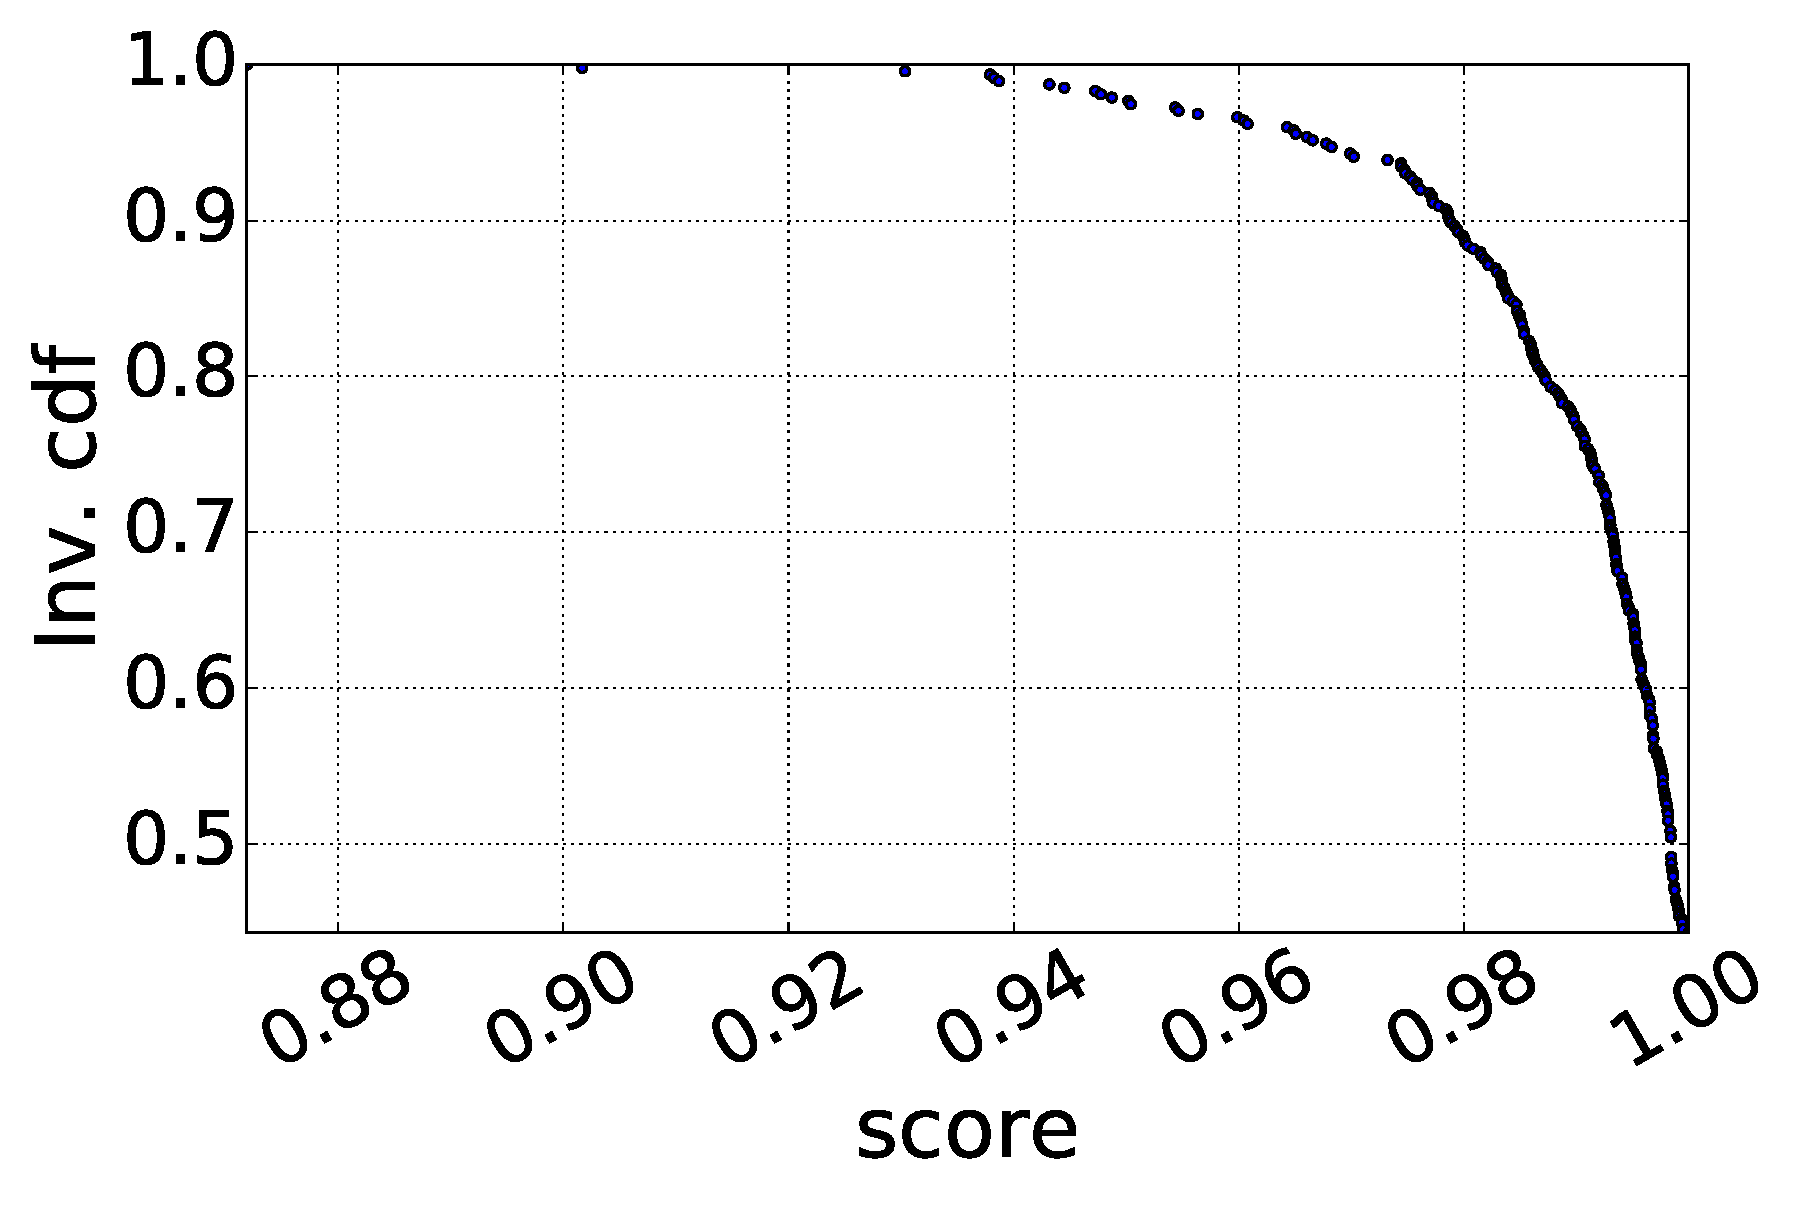
\includegraphics[width=\linewidth]{img/GroupeDense/#1/Percentil/Distribution_percentil_Rand_top155.eps}
		\caption{N\oe uds:$p_{noeuds}$}
	\end{subfigure}\hfill
	\caption{Distribution cumulative inverse des scores pour chaque voisinage dans le jeu de données #2.}
	\label{fig:dit_#3}
	\end{figure}
}

\newcommand{\correlation}[4]{
	\begin{figure}[#4]
	\centering
	
	\begin{subfigure}{\largeurGroupeDense\linewidth}
		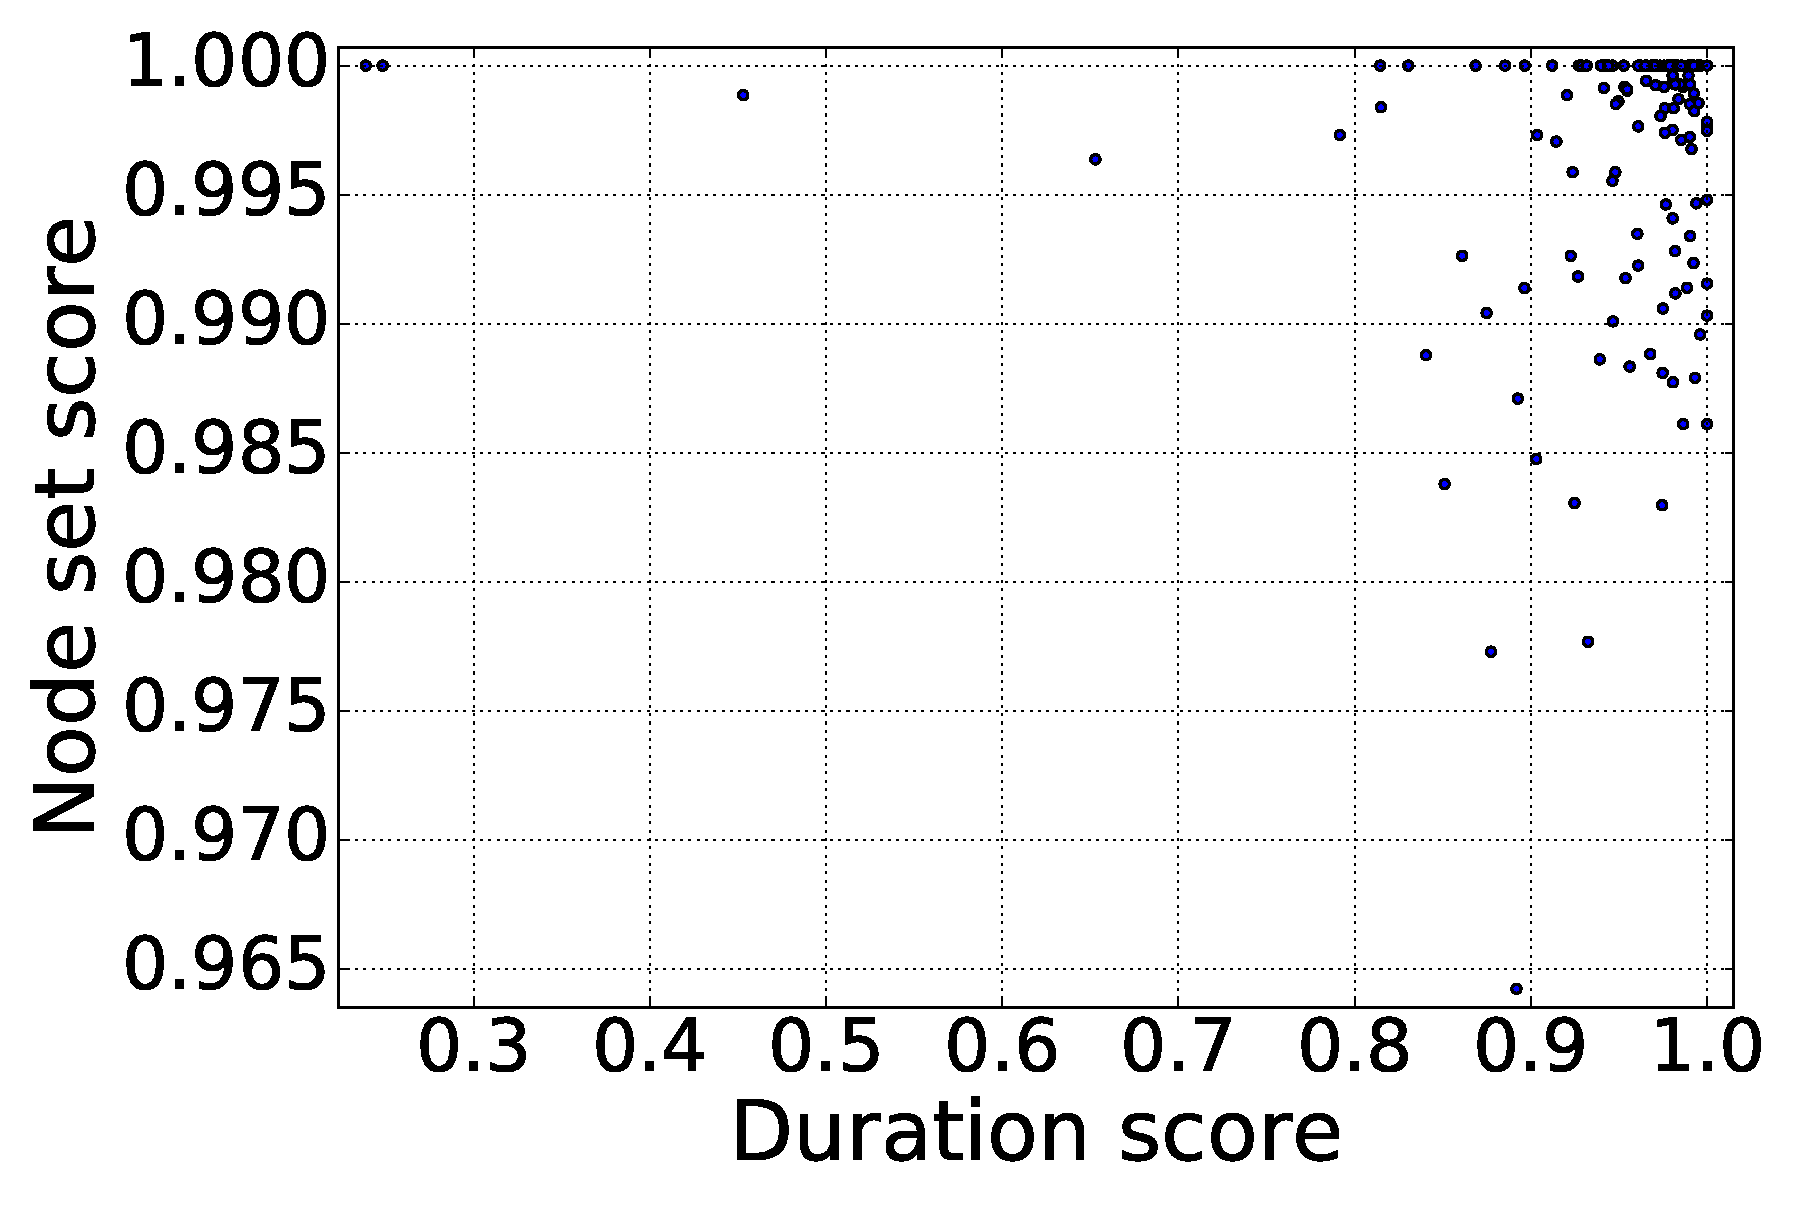
\includegraphics[width=\linewidth]{img/GroupeDense/#1/ecart/relationFixTime_Rand}
		\caption{} %Corrélation entre les score au temps de début et aux n\oe uds.}
	\end{subfigure}\hfill
	\begin{subfigure}{\largeurGroupeDense\linewidth}
		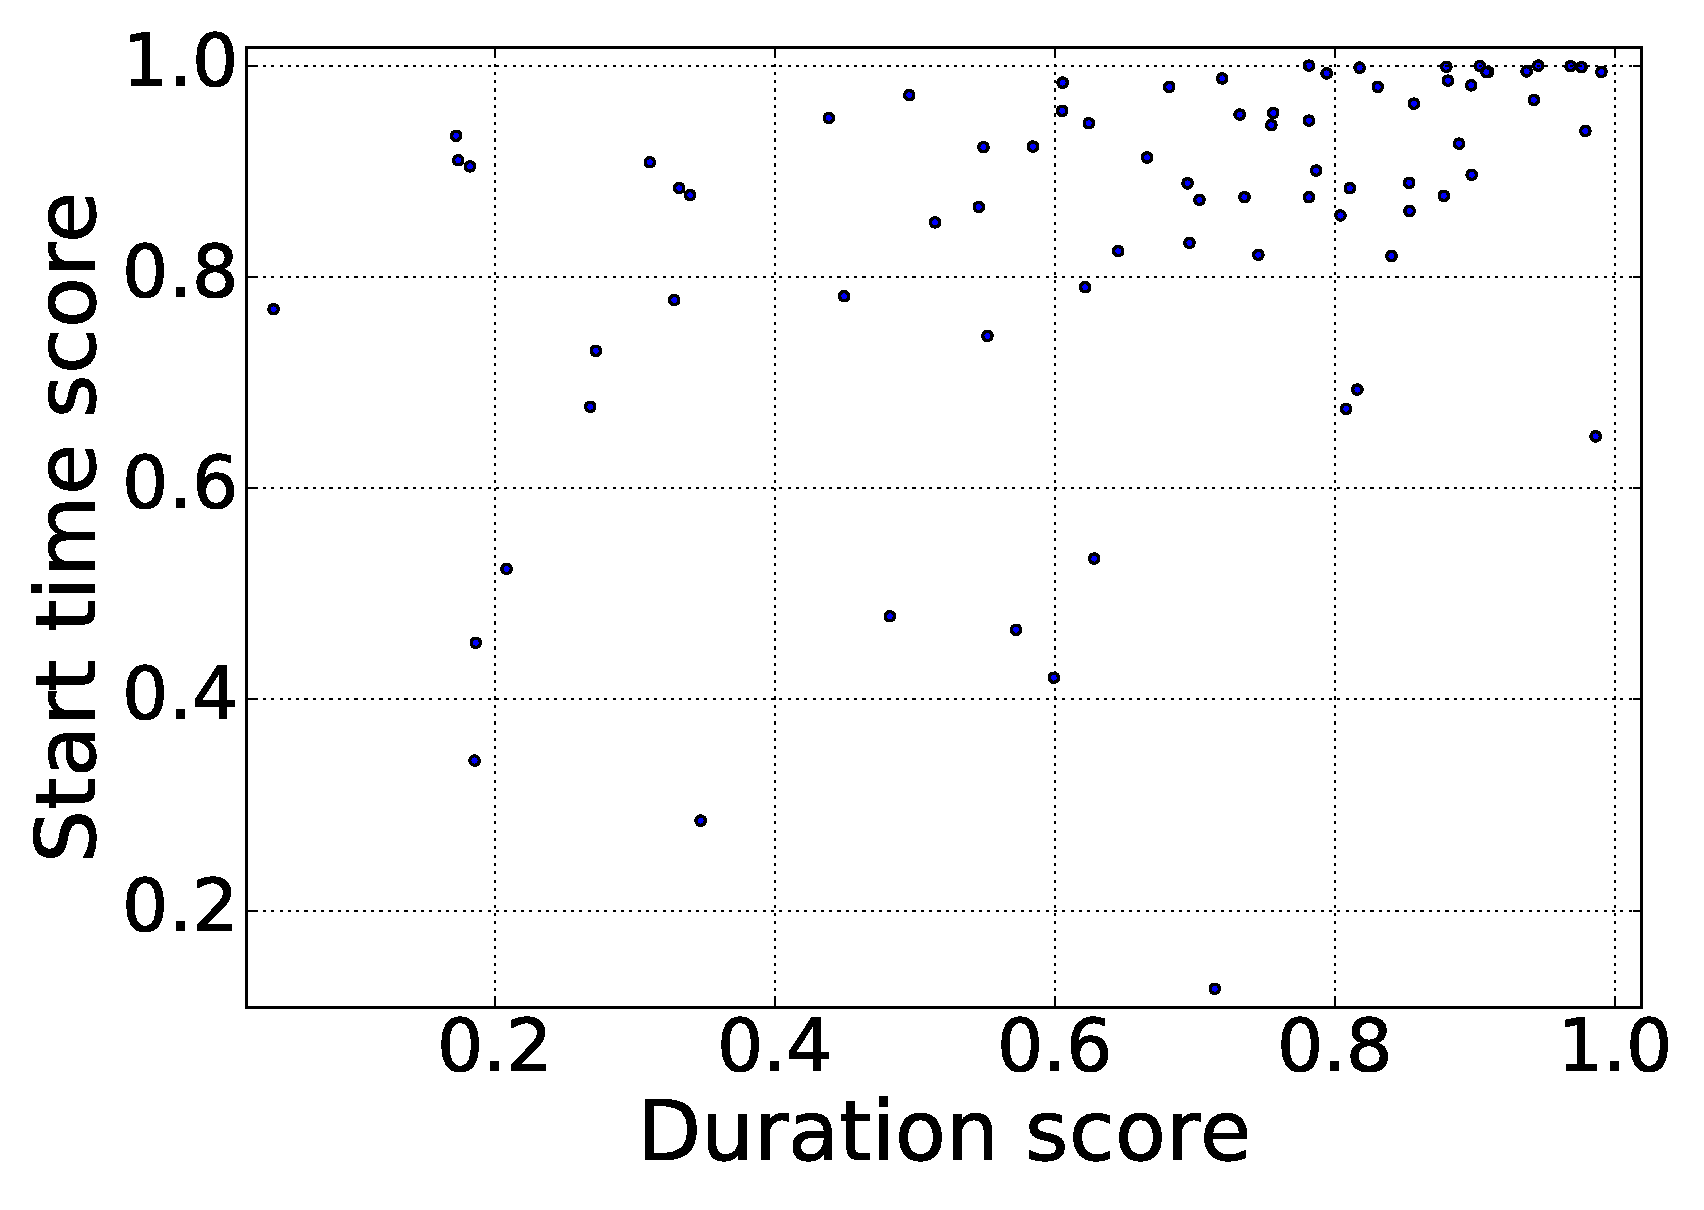
\includegraphics[width=\linewidth]{img/GroupeDense/#1/ecart/relationFixTime_FixDuration.eps}
		\caption{}%Corrélation entre les score au temps de début et à la durée.}
	\end{subfigure}\hfill
	\begin{subfigure}{\largeurGroupeDense\linewidth}
		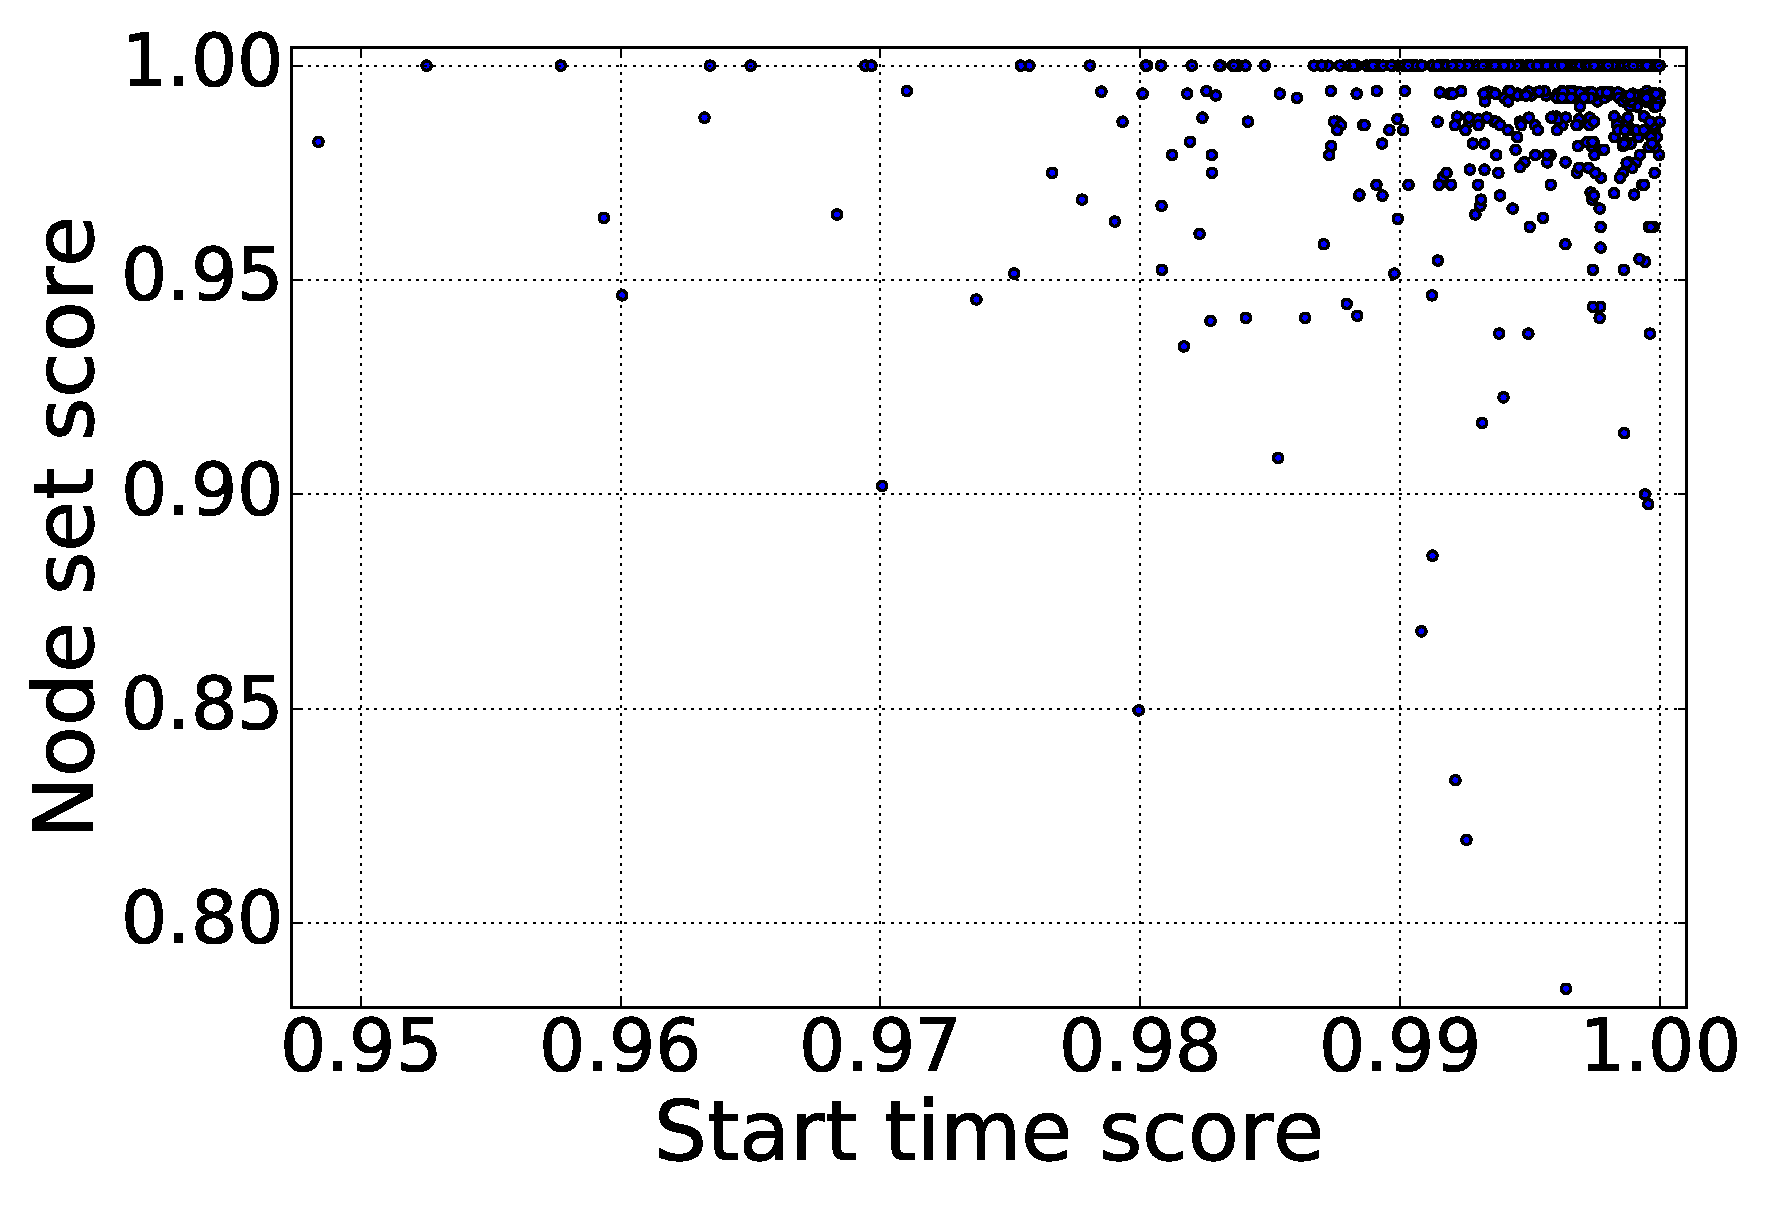
\includegraphics[width=\linewidth]{img/GroupeDense/#1/ecart/relationFixDuration_Rand.eps}
		\caption{} %Corrélation entre les score aux n\oe uds et à la durée.}
	\end{subfigure}
	\caption{Corrélations des scores selon le voisinage dans le jeu de données #2.}
	\label{fig:correlation_#3}
	\end{figure}
}

\newcommand{\groupcharacFilter}[4]{
	\begin{figure}[#4]
	\centering
	
	\begin{subfigure}{\largeurGroupeDense\linewidth}
		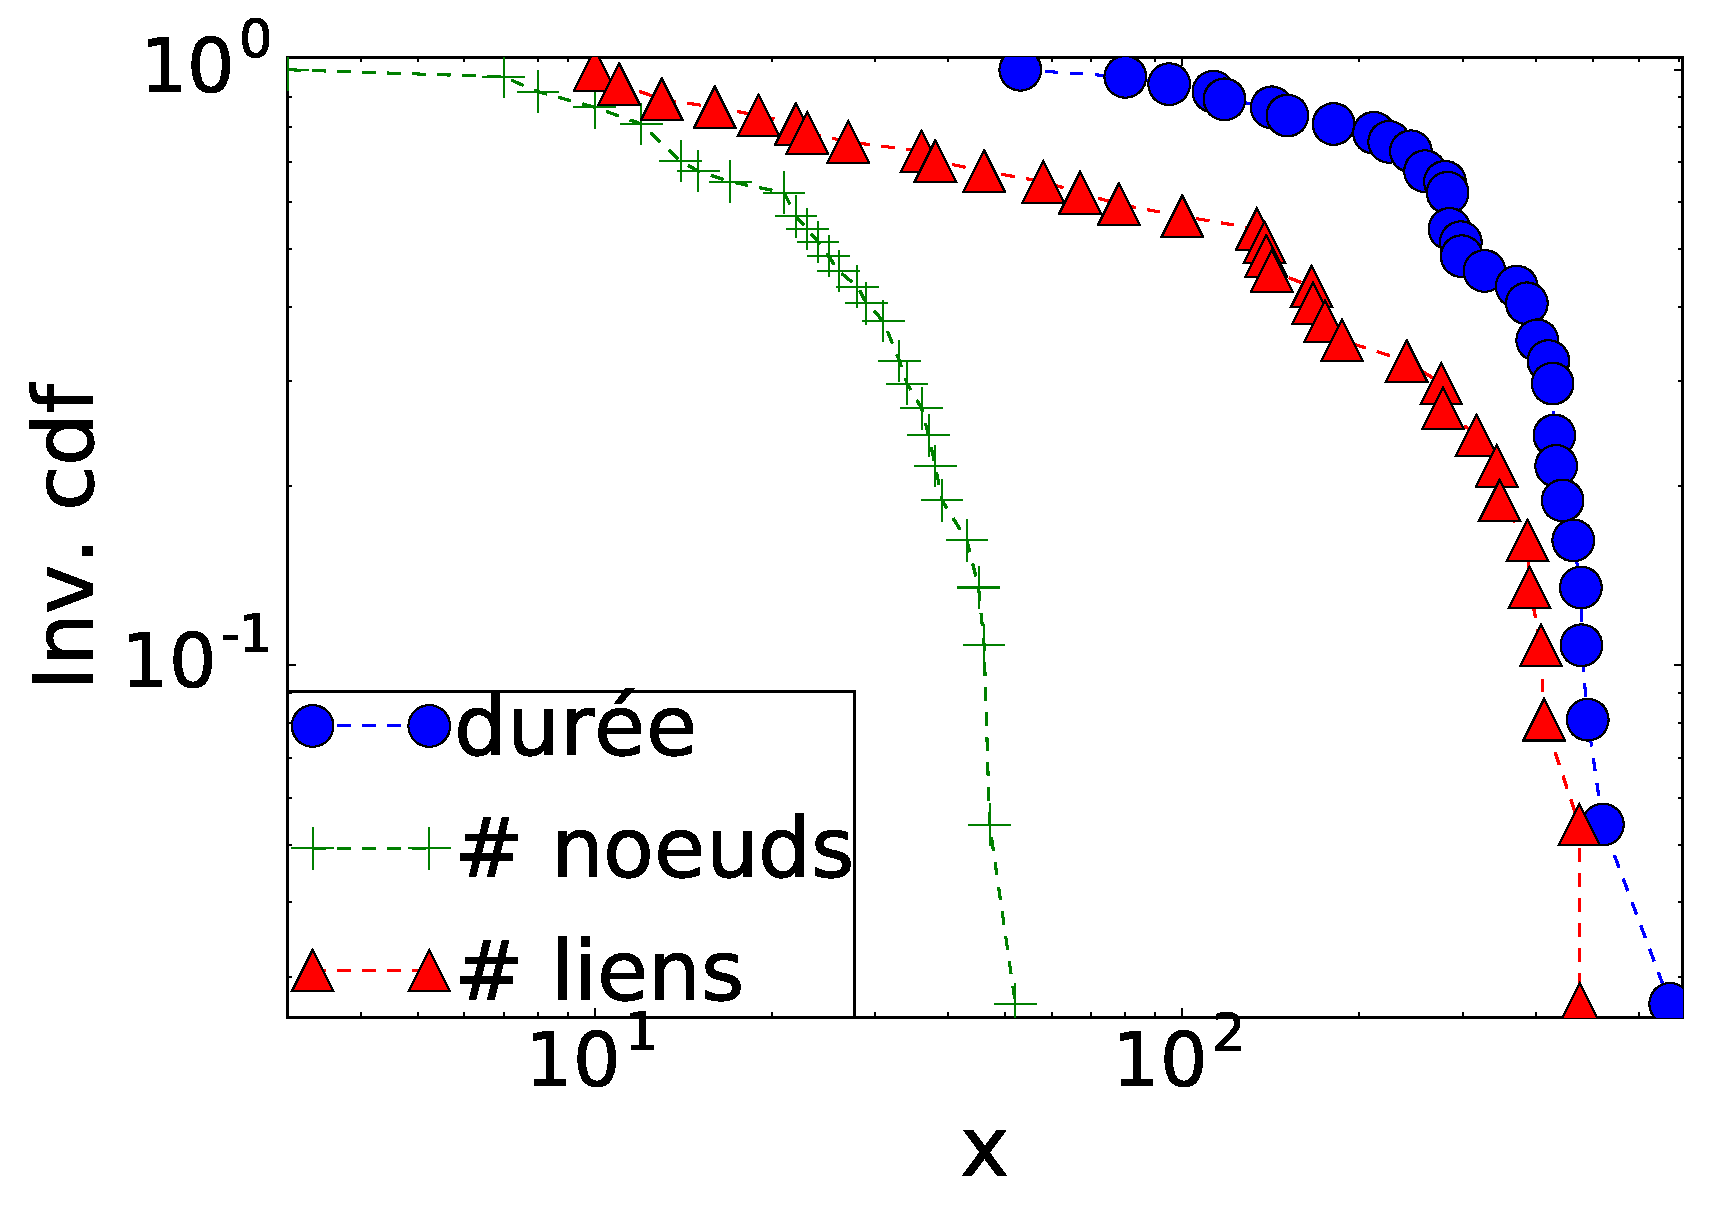
\includegraphics[width=\linewidth]{img/GroupeDense/#1/filter/Distrib_apres_filtre_best}
		\caption{}
	\end{subfigure}\hfill
	\begin{subfigure}{\largeurGroupeDense\linewidth}
		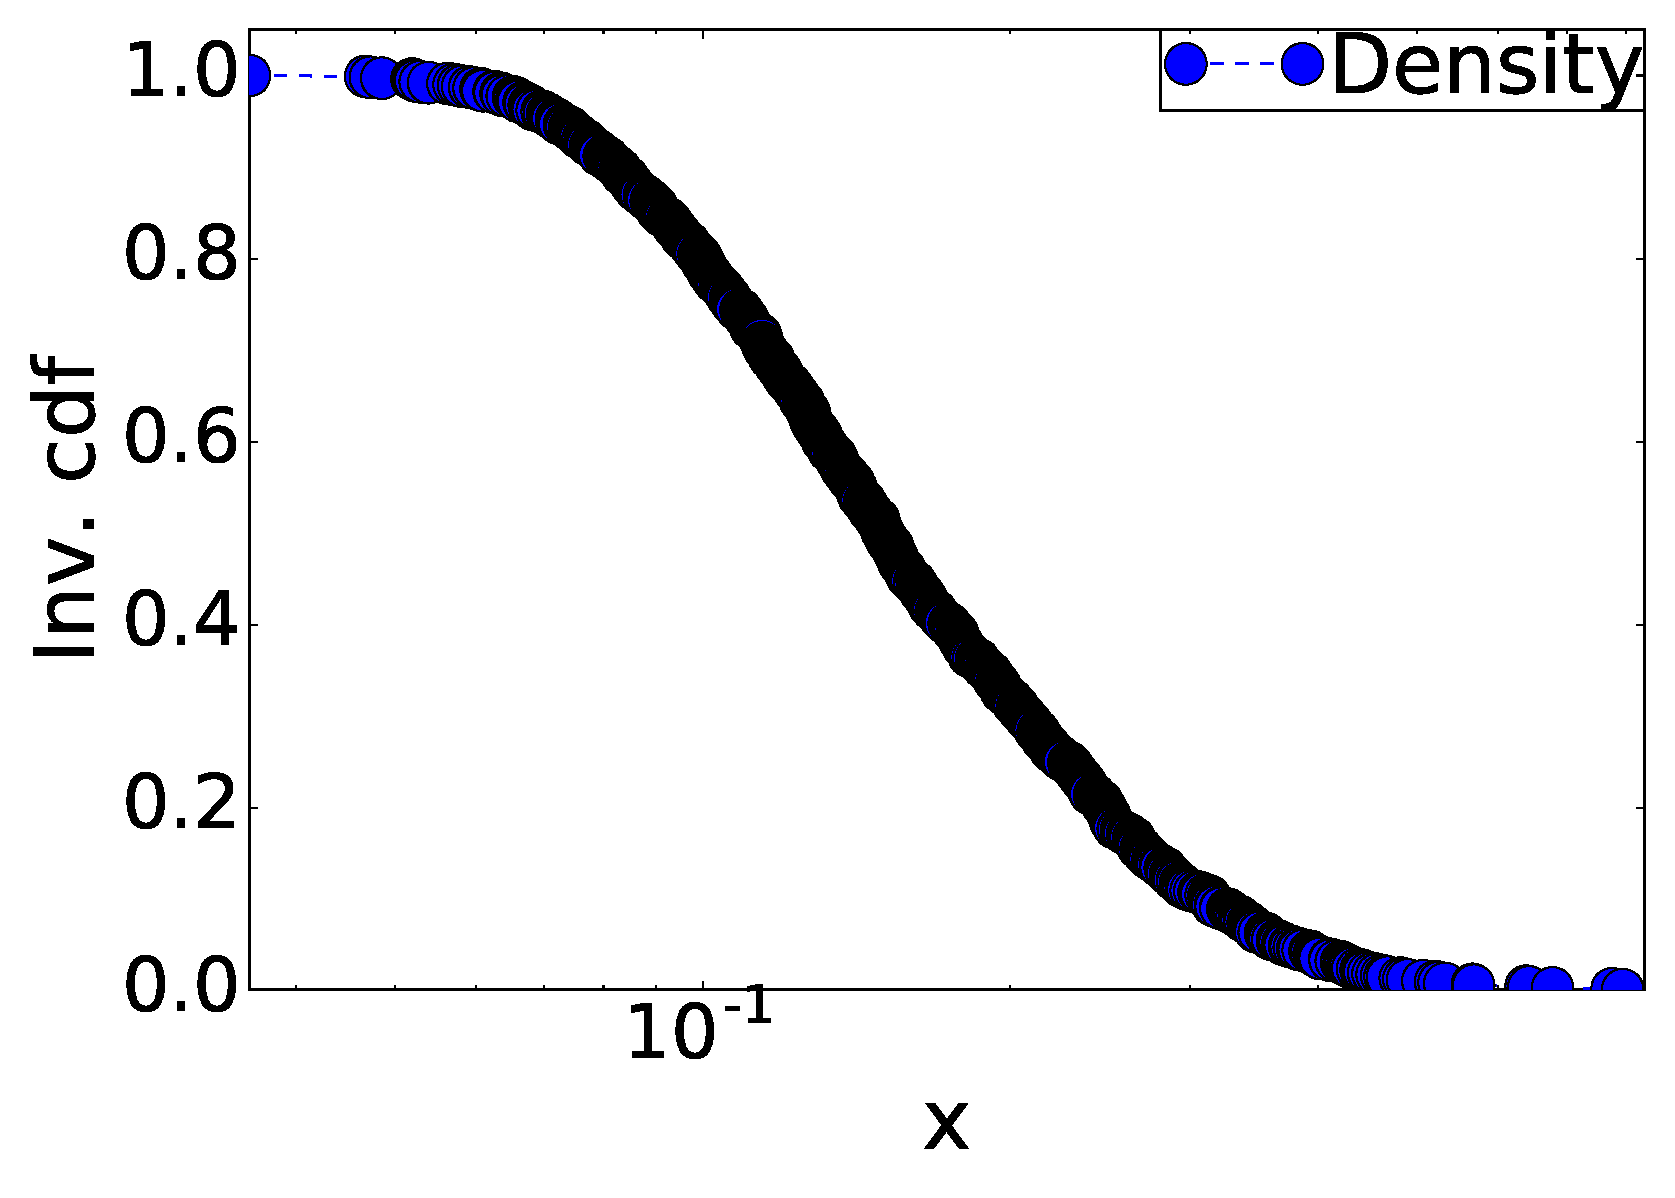
\includegraphics[width=\linewidth]{img/GroupeDense/#1/filter/Distrib_apres_dens.eps}
		\caption{}
	\end{subfigure}\hfill
	\begin{subfigure}{\largeurGroupeDense\linewidth}
			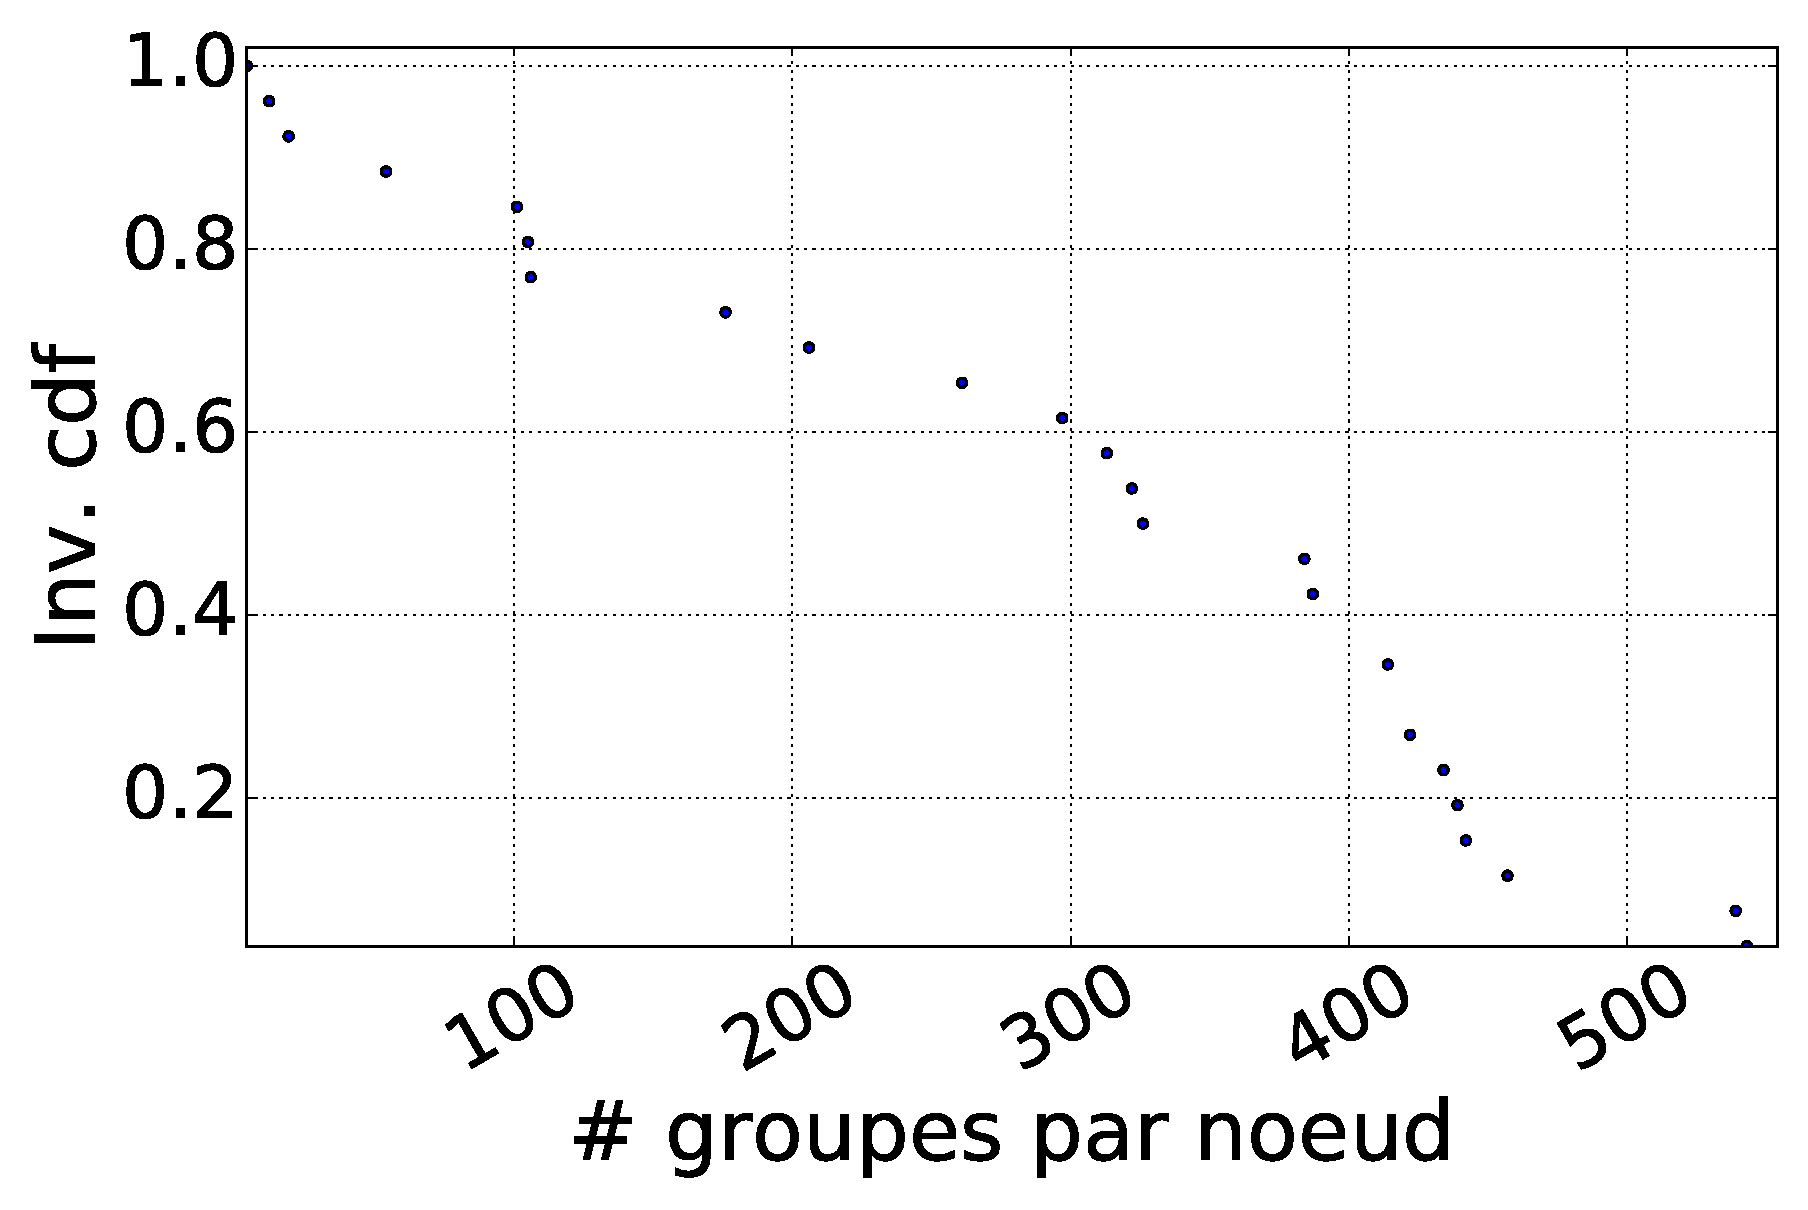
\includegraphics[width=\linewidth]{img/GroupeDense/#1/filter/Prop_node.eps}
			\caption{}
			\label{fig:PropNode_#3}
	\end{subfigure}
	\caption{Distributions cumulatives inverses du nombre de liens, de n\oe uds et de la durée en (A), de la densité en (B), du nombre de groupes par n\oe ud en (C) pour les groupes capturés par notre méthode dans les données #2.}
	\label{fig:distri_group_#3_filter}
	\end{figure}
}

%----------------------------------------------------------------------------------------
%	MARGIN SETTINGS
%----------------------------------------------------------------------------------------

\geometry{
	paper=a4paper, % Change to letterpaper for US letter
	inner=1.5cm, % Inner margin
	outer=2.5cm, % Outer margin
	bindingoffset=1cm, % Binding offset
	top=1.5cm, % Top margin
	bottom=1.5cm, % Bottom margin
	%showframe,% show how the type block is set on the page
}

%----------------------------------------------------------------------------------------
%	THESIS INFORMATION
%----------------------------------------------------------------------------------------
\dominitoc

\thesistitle{Conversations, Groupes et Communautés dans les Flots de Liens} % Your thesis title, this is used in the title and abstract, print it elsewhere with \ttitle
\supervisor{Clémence \textsc{Magnien}\\ Matthieu \textsc{Latapy}} % Your supervisor's name, this is used in the title page, print it elsewhere with \supname
\examiner{..} % Your examiner's name, this is not currently used anywhere in the template, print it elsewhere with \examname
\degree{Doctor of Philosophy} % Your degree name, this is used in the title page and abstract, print it elsewhere with \degreename
\author{Noé \textsc{Gaumont}} % Your name, this is used in the title page and abstract, print it elsewhere with \authorname
\addresses{} % Your address, this is not currently used anywhere in the template, print it elsewhere with \addressname

\subject{... Sciences} % Your subject area, this is not currently used anywhere in the template, print it elsewhere with \subjectname
\keywords{} % Keywords for your thesis, this is not currently used anywhere in the template, print it elsewhere with \keywordnames
\university{\href{http://www.university.com}{University Name}} % Your university's name and URL, this is used in the title page and abstract, print it elsewhere with \univname
\department{\href{http://department.university.com}{Department or School Name}} % Your department's name and URL, this is used in the title page and abstract, print it elsewhere with \deptname
\group{\href{http://researchgroup.university.com}{Research Group Name}} % Your research group's name and URL, this is used in the title page, print it elsewhere with \groupname
\faculty{\href{http://faculty.university.com}{Faculty Name}} % Your faculty's name and URL, this is used in the title page and abstract, print it elsewhere with \facname

\hypersetup{pdftitle=\ttitle} % Set the PDF's title to your title
\hypersetup{pdfauthor=\authorname} % Set the PDF's author to your name
\hypersetup{pdfkeywords=\keywordnames} % Set the PDF's keywords to your keywords

\newcommand{\REF}{\textcolor{red}{REF}}
\newcommand{\com}[1]{\textcolor{red}{#1} }



